\section{Experimental Results}
In this section, we apply the proposed framework to multiple COVID-19 datasets, all of which are daily and at the state level. These datasets, available to the Delphi Group, vary in source, format, and update frequency. Furthermore, each dataset exhibits a unique data revision pattern, making the performance of the framework across different datasets not directly comparable.

\subsection{Description of Datasets}
\paragraph{Insurance Claims:} We use insurance claims data provided by Change Healthcare (CHNG). CHNG aggregates claim data from numerous healthcare providers and payers, and the information provided by CHNG spans more than two thousand of the most populous US counties, covering more than 45\% of the total US population. Our analysis focuses on a time series comprising the aggregate count of claims featuring ICD codes indicative of COVID-19 diagnoses recorded daily within each county. The reference date corresponds to the claim's date of service, while the report date denotes its appearance in the CHNG database, which may vary considerably depending on providers' claim filing times. Sometimes, Delphi receives the initial report release for a reference date on the same day. We produce forecasts for each reference date between 2021-06-01 and 2023-01-10 (a total of 589 days including the Delta wave and the Omicron wave of COVID-19). 

\paragraph{Antigen Tests:}
This dataset is provided by Quidel Corporation (Quidel), which supplies devices used by healthcare providers to conduct COVID-19 antigen tests. We construct a time series of the fraction of positive tests using this dataset. The test records indicate the test date (when the test was conducted) and storage date (when the test was logged into Quidel's MyVirena cloud storage system). The test date serves as the reference date, and test records with a storage date preceding the test date or more than 90 days after are excluded. The report date is defined as the date the records are shared with the Delphi Group via a cloud platform. Typically, Quidel releases the initial report for each reference date on the following day (lag = 1), at the earliest. We produce forecasts for all the states and reference dates ranging from 2021-05-18 to 2022-12-12 (a total of 574 days). 

\paragraph{COVID-19 Cases in MA:}
The Massachusetts Department of Public Health (MA-DPH) provides a comprehensive revision history of COVID-19 case reporting. This dataset includes the 7-day moving average of confirmed COVID-19 cases, updated daily from 2021-01-01, until 2022-07-08. After this date, the reporting frequency transitioned to weekly updates, occurring every Thursday. The first release of the report for a reference date \( t \) is usually made on date \( t+1 \). A distinctive feature of this dataset is that the COVID-19 confirmed cases are usually normalized by the population, which is large enough to render fluctuations over extended periods negligible compared to the numerators. In contrast, the fractional denominators in the other two datasets exhibit noticeable revision sequences, similar to the numerators. We used data reported before 2022-07-08, and produced forecasts for reference dates ranging from 2021-04-01, to 2022-06-24 (a span of 450 days).


\subsection{Data Processing}

\paragraph{Data Filtering:}
All datasets are filtered based on the specified time period to ensure data quality. For CHNG outpatient insurance claim data and Quidel antigen test data, this filtering process excludes periods affected by prolonged data reporting issues, such as significant declines in report volume over several months. These anomalies, which may present as abrupt shifts in data distribution, do not indicate 'real' changes in data revision patterns but rather indicate data quality issues. The MA-DPH case data are filtered to include only the period with consistent daily reporting. As shown in Figure 1, over 90\% of the confirmed cases for a given reference date are reported within 7 days. Given this pattern, developing a data revision forecasting model for weekly reports is unnecessary.

\paragraph{Missing data imputation:}
Before integrating the data into our framework, we address missing data according to the definition explained in preliminaries. Specifically, for the epidemic count of interest $Y_{it}$ associated with location $i$ and reference date $t$, if $Y_{it}$ has never been reported yet, we assume that there are historical reports of 0 (s). If it has not been reported on a particular report date $s$ ($Y_{it(s-t)}$=NA), we use the latest report in the data revision sequence of $Y_{it}$ as its report for date $s$. 

\subsection{Experimental Setup}
\begin{figure}[h!]
    \centering
    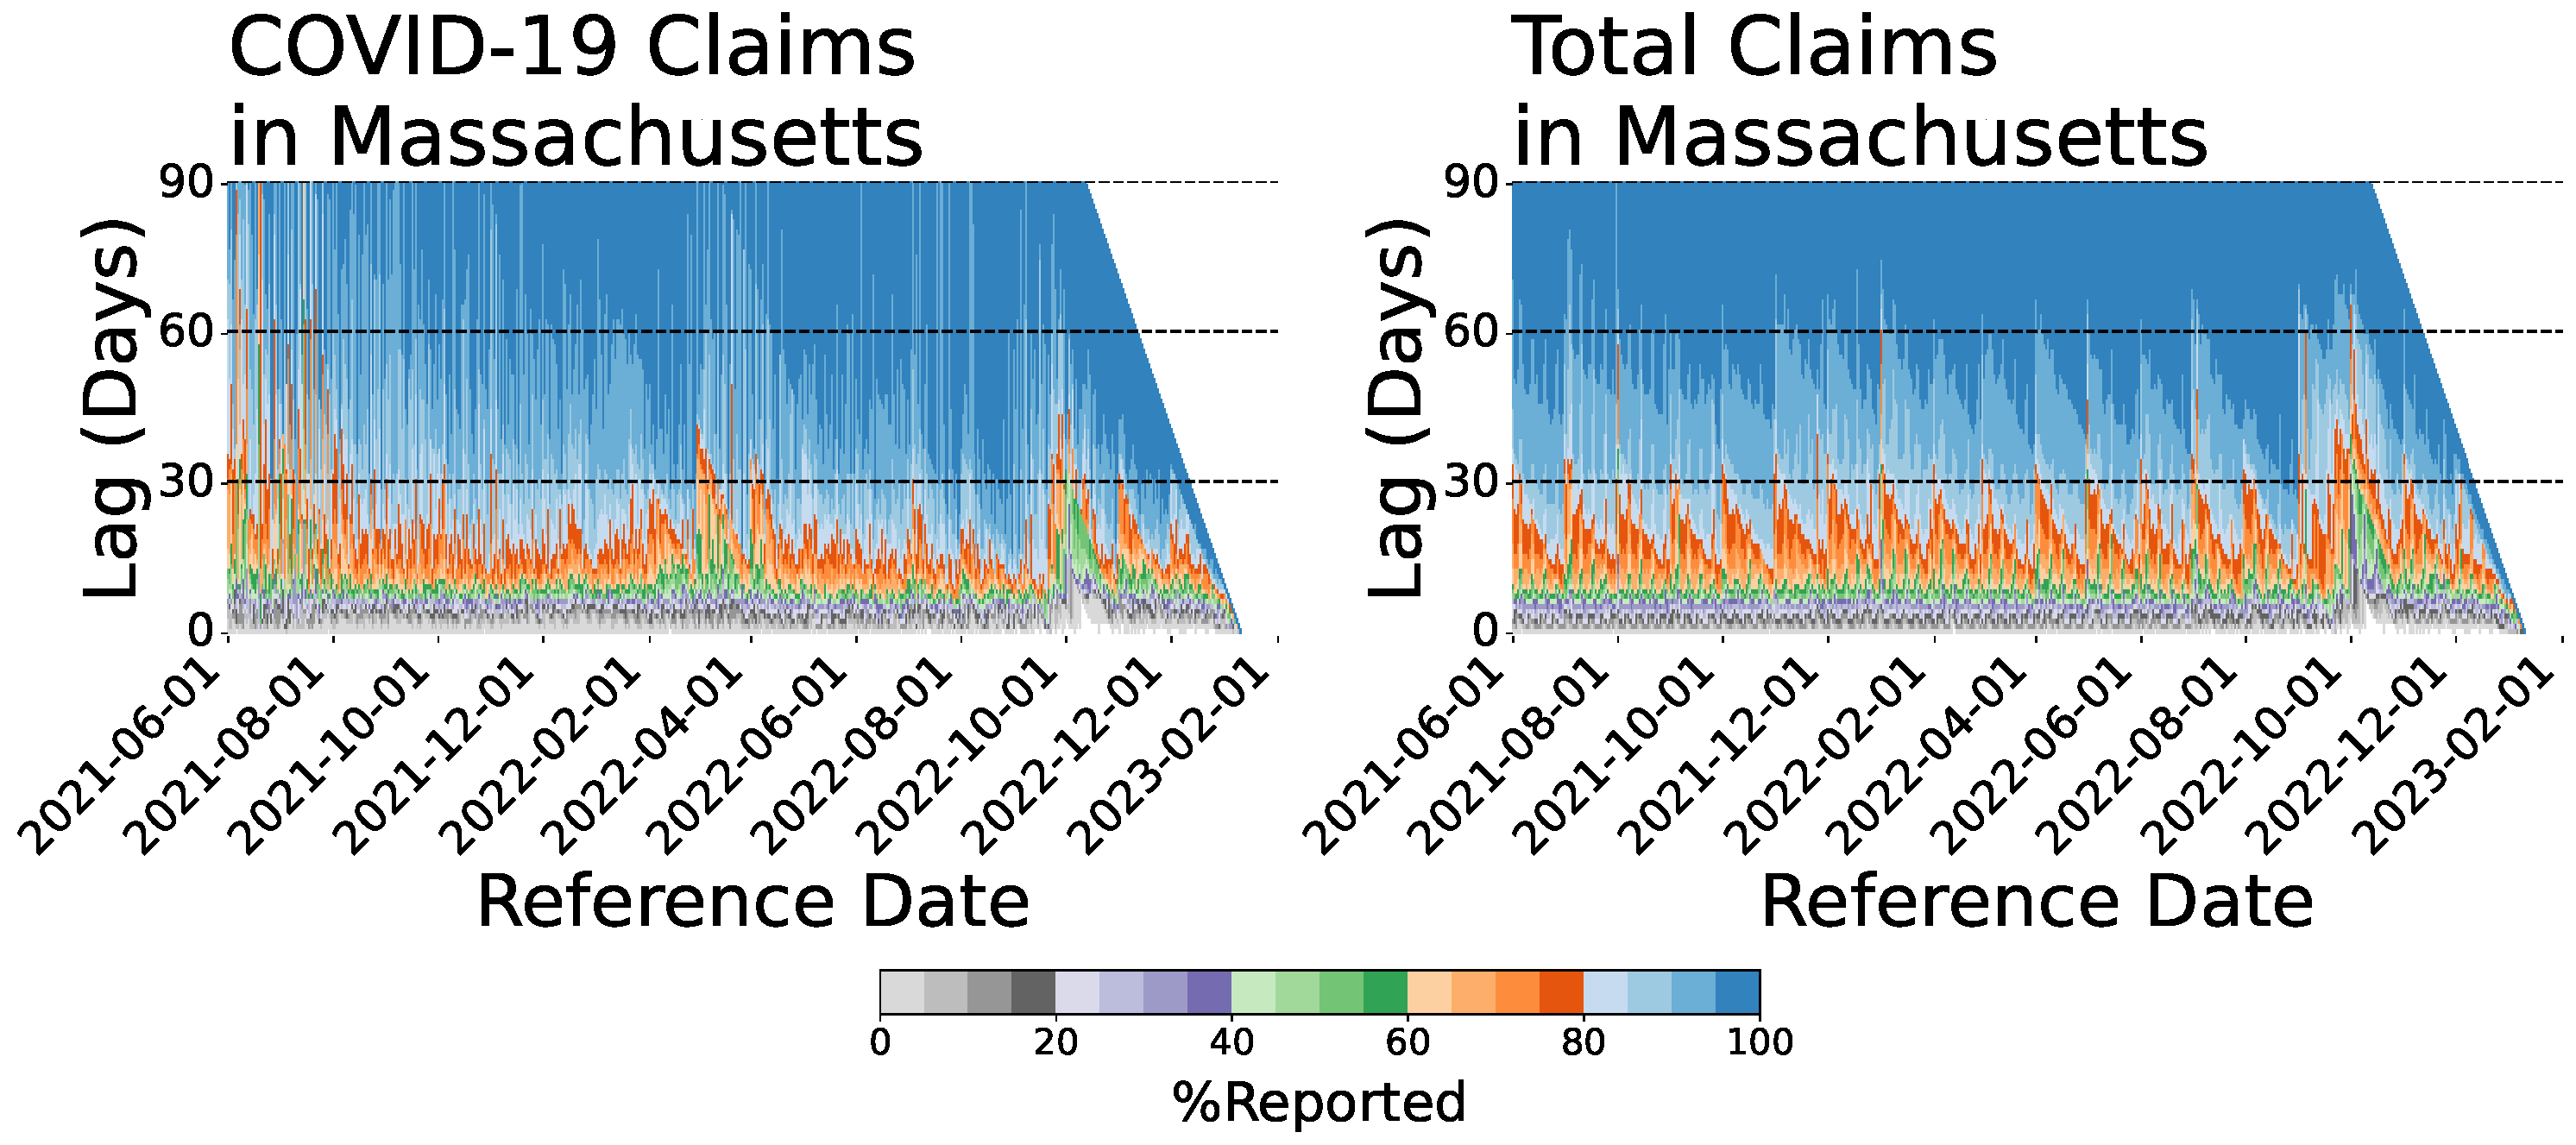
\includegraphics[width=\textwidth]{figs/completeness_Massachusetts.pdf}
    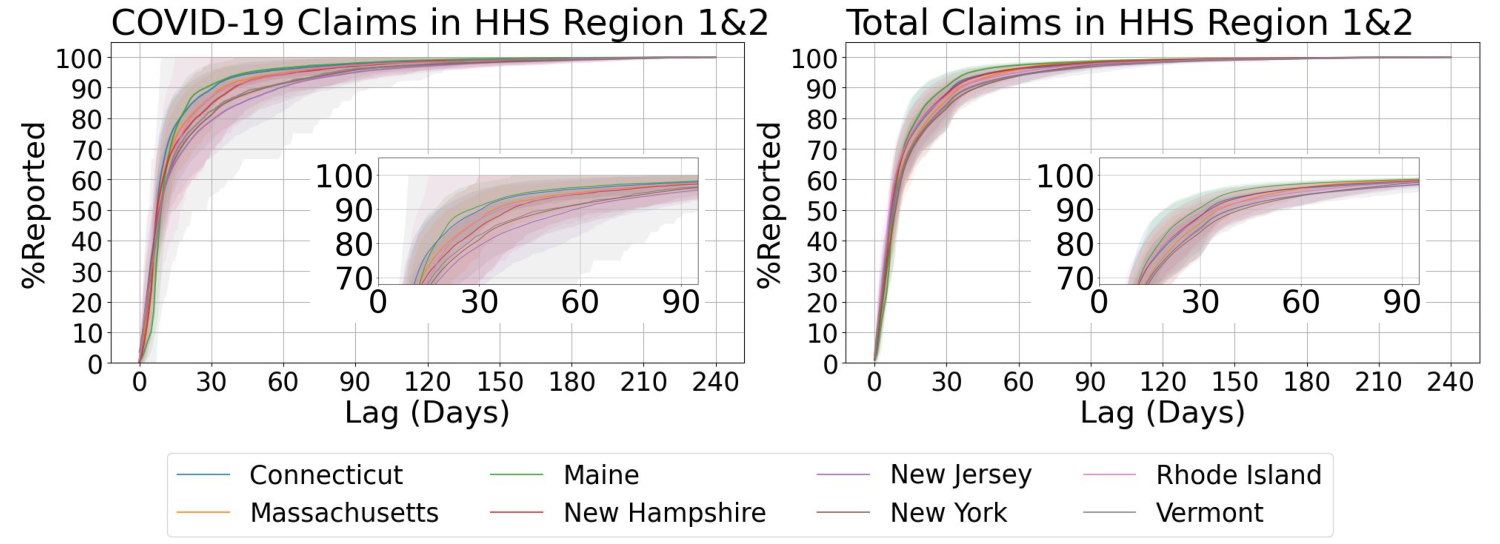
\includegraphics[width=\textwidth]{figs/completeness_lineplot_hhs1&2.pdf}
    \caption{\emph{Top: percentage of reported distribution in Massachusetts, grouped by lag, and recorded over reference dates. Bottom: Mean percentage of reported, averaged over all reference dates between 2021-04-01 and 2023-01-10, over lags for states in HHS Region 1\&2. The shaded bands correspond to 10\% quantile to 90\% quantile intervals. The left panel in the figure is based on CHNG outpatient COVID-19 claims data while the right panel is based on CHNG outpatient total claims data.}}
\end{figure}

\paragraph{Selection of Target Tag $L$:}
A useful way we propose to look at the data revision pattern is by examining the distribution of variable $p_{itl}$ defined as $p_{itl} = \frac{Y_{itl}}{Y_{it}}$
over lag. 
When the value type of $Y_{itl}$ is counted (for example, the number of confirmed cases), $p_{itl} \time 100$ describes the percentage of claims that have been reported after the $(l+1)$th release for location $i$ and reference date $t$. When the value type of $Y_{itl}$ is a fraction (for example, the fraction of COVID-19 insurance claims), $p_{itl}$ describes the normalized provisional fraction. Given that $Y_{it}$ is continually revised and asymptotic, we temporarily use $Y_{itl_m}$ (with $l_m = 300$, which is large enough for $Y_{it}$ to nearly converge) as an approximation. 



The distribution of $p_{itl}$ provides insight into how data revision sequences evolve over time. In addition to the apparent day-of-week effect and week-of-month effect, the efficiency of data revision is significantly influenced during periods when the epidemic curve is at or near its peak. Figure 2 illustrates this phenomenon using CHNG outpatient insurance claim data in Massachusetts as an example. Overall, the revision of COVID-19 claims exhibit greater variance than non-COVID claims, underscoring the difficulty of the forecast task.

Although there may be a considerable degree of heterogeneity in $L_{it}$ (the target horizon for $Y_{it}$, example shown in Figure S1 in the appendix), the most substantial revisions are typically made within the first two months for the majority locations including states and populous counties for all the three datasets considered. The bottom panel of Figure 2 shows an example based on CHNG outpatient COVID-19 insurance claims data. It reveals that, for states in HHS Region 1 and Region 2, almost all mean \%reported values for COVID-19 reach 90\% when the lag equals 60.  

In our experiments, we set $L=60$ for CHNG outpatient COVID-19 claims data, $L=45$ for Quidel COVID-19 antigen test data and $L=14$ for confirmed case data from MA-DPH to ensure that at least 90\% counts are reported while keeping $L$ relatively small. 

\paragraph{Training Frequency:}
We generate forecasts at the state level following the adaptive modeling protocol outlined in Section 4.3. However, for computational efficiency, we adjust the model training frequency to occur every 30 days, with the exception of MA-DPH case forecasting, for which the model is trained every 7 days. This adjustment increases the risk of introducing bias, particularly in scenarios with abrupt and significant changes in data revision patterns. On each test date \( S \), we generate quantile forecasts based on all epidemic quantities reported on dates \( s \in (S-30, S] \) (\( s \in (S-7, S] \) for the MA-DPH case forecast) and assess the forecast error as a function of lag at which the forecasts are made.


\paragraph{Location-Specific Model Training:}
Both of CHNG insurance claims data and Quidel antigen test data are subject to geographic differences in market share, health-seeking behavior, and data-reporting behavior, which makes the data not comparable across different geographic locations. In the current paper, we do not attempt to address the issue of spatial heterogeneity, and we simply fit the model per location.








